\documentclass[11pt,preprint]{elsarticle}

\usepackage{lmodern}
%%%% My spacing
\usepackage{setspace}
\setstretch{1.2}
\DeclareMathSizes{12}{14}{10}{10}

% Wrap around which gives all figures included the [H] command, or places it "here". This can be tedious to code in Rmarkdown.
\usepackage{float}
\let\origfigure\figure
\let\endorigfigure\endfigure
\renewenvironment{figure}[1][2] {
    \expandafter\origfigure\expandafter[H]
} {
    \endorigfigure
}

\let\origtable\table
\let\endorigtable\endtable
\renewenvironment{table}[1][2] {
    \expandafter\origtable\expandafter[H]
} {
    \endorigtable
}


\usepackage{ifxetex,ifluatex}
\usepackage{fixltx2e} % provides \textsubscript
\ifnum 0\ifxetex 1\fi\ifluatex 1\fi=0 % if pdftex
  \usepackage[T1]{fontenc}
  \usepackage[utf8]{inputenc}
\else % if luatex or xelatex
  \ifxetex
    \usepackage{mathspec}
    \usepackage{xltxtra,xunicode}
  \else
    \usepackage{fontspec}
  \fi
  \defaultfontfeatures{Mapping=tex-text,Scale=MatchLowercase}
  \newcommand{\euro}{€}
\fi

\usepackage{amssymb, amsmath, amsthm, amsfonts}

\def\bibsection{\section*{References}} %%% Make "References" appear before bibliography


\usepackage[numbers]{natbib}

\usepackage{longtable}
\usepackage[margin=2.3cm,bottom=2cm,top=2.5cm, includefoot]{geometry}
\usepackage{fancyhdr}
\usepackage[bottom, hang, flushmargin]{footmisc}
\usepackage{graphicx}
\numberwithin{equation}{section}
\numberwithin{figure}{section}
\numberwithin{table}{section}
\setlength{\parindent}{0cm}
\setlength{\parskip}{1.3ex plus 0.5ex minus 0.3ex}
\usepackage{textcomp}
\renewcommand{\headrulewidth}{0.2pt}
\renewcommand{\footrulewidth}{0.3pt}

\usepackage{array}
\newcolumntype{x}[1]{>{\centering\arraybackslash\hspace{0pt}}p{#1}}

%%%%  Remove the "preprint submitted to" part. Don't worry about this either, it just looks better without it:
\makeatletter
\def\ps@pprintTitle{%
  \let\@oddhead\@empty
  \let\@evenhead\@empty
  \let\@oddfoot\@empty
  \let\@evenfoot\@oddfoot
}
\makeatother

 \def\tightlist{} % This allows for subbullets!

\usepackage{hyperref}
\hypersetup{breaklinks=true,
            bookmarks=true,
            colorlinks=true,
            citecolor=blue,
            urlcolor=blue,
            linkcolor=blue,
            pdfborder={0 0 0}}


% The following packages allow huxtable to work:
\usepackage{siunitx}
\usepackage{multirow}
\usepackage{hhline}
\usepackage{calc}
\usepackage{tabularx}
\usepackage{booktabs}
\usepackage{caption}


\newenvironment{columns}[1][]{}{}

\newenvironment{column}[1]{\begin{minipage}{#1}\ignorespaces}{%
\end{minipage}
\ifhmode\unskip\fi
\aftergroup\useignorespacesandallpars}

\def\useignorespacesandallpars#1\ignorespaces\fi{%
#1\fi\ignorespacesandallpars}

\makeatletter
\def\ignorespacesandallpars{%
  \@ifnextchar\par
    {\expandafter\ignorespacesandallpars\@gobble}%
    {}%
}
\makeatother


% definitions for citeproc citations
\NewDocumentCommand\citeproctext{}{}
\NewDocumentCommand\citeproc{mm}{%
\href{\#cite.\detokenize{#1}}{#2}\nocite{#1}}

\makeatletter
% allow citations to break across lines
\let\@cite@ofmt\@firstofone
% avoid brackets around text for \cite:
\def\@biblabel#1{}
\def\@cite#1#2{{#1\if@tempswa , #2\fi}}
\makeatother
\newlength{\cslhangindent}
\setlength{\cslhangindent}{1.5em}
\newlength{\csllabelwidth}
\setlength{\csllabelwidth}{3em}
\newenvironment{CSLReferences}[2] % #1 hanging-indent, #2 entry-spacing
{\begin{list}{}{%
	\setlength{\itemindent}{0pt}
	\setlength{\leftmargin}{0pt}
	\setlength{\parsep}{0pt}
	% turn on hanging indent if param 1 is 1
	\ifodd #1
	\setlength{\leftmargin}{\cslhangindent}
	\setlength{\itemindent}{-1\cslhangindent}
	\fi
	% set entry spacing
	\setlength{\itemsep}{#2\baselineskip}}}
{\end{list}}

\usepackage{calc}
\newcommand{\CSLBlock}[1]{\hfill\break\parbox[t]{\linewidth}{\strut\ignorespaces#1\strut}}
\newcommand{\CSLLeftMargin}[1]{\parbox[t]{\csllabelwidth}{\strut#1\strut}}
\newcommand{\CSLRightInline}[1]{\parbox[t]{\linewidth - \csllabelwidth}{\strut#1\strut}}
\newcommand{\CSLIndent}[1]{\hspace{\cslhangindent}#1}


\urlstyle{same}  % don't use monospace font for urls
\setlength{\parindent}{0pt}
\setlength{\parskip}{6pt plus 2pt minus 1pt}
\setlength{\emergencystretch}{3em}  % prevent overfull lines
\setcounter{secnumdepth}{5}

%%% Use protect on footnotes to avoid problems with footnotes in titles
\let\rmarkdownfootnote\footnote%
\def\footnote{\protect\rmarkdownfootnote}
\IfFileExists{upquote.sty}{\usepackage{upquote}}{}

%%% Include extra packages specified by user
\usepackage{colortbl}
\usepackage{graphicx}
\usepackage{adjustbox}
\usepackage{framed}
\usepackage{fancyvrb}
\DefineVerbatimEnvironment{Shaded}{Verbatim}{frame=single}\usepackage{booktabs}
\usepackage{longtable}
\usepackage{array}
\usepackage{multirow}
\usepackage{wrapfig}
\usepackage{float}
\usepackage{colortbl}
\usepackage{pdflscape}
\usepackage{tabu}
\usepackage{threeparttable}
\usepackage{threeparttablex}
\usepackage[normalem]{ulem}
\usepackage{makecell}
\usepackage{xcolor}

%%% Hard setting column skips for reports - this ensures greater consistency and control over the length settings in the document.
%% page layout
%% paragraphs
\setlength{\baselineskip}{12pt plus 0pt minus 0pt}
\setlength{\parskip}{12pt plus 0pt minus 0pt}
\setlength{\parindent}{0pt plus 0pt minus 0pt}
%% floats
\setlength{\floatsep}{12pt plus 0 pt minus 0pt}
\setlength{\textfloatsep}{20pt plus 0pt minus 0pt}
\setlength{\intextsep}{14pt plus 0pt minus 0pt}
\setlength{\dbltextfloatsep}{20pt plus 0pt minus 0pt}
\setlength{\dblfloatsep}{14pt plus 0pt minus 0pt}
%% maths
\setlength{\abovedisplayskip}{12pt plus 0pt minus 0pt}
\setlength{\belowdisplayskip}{12pt plus 0pt minus 0pt}
%% lists
\setlength{\topsep}{10pt plus 0pt minus 0pt}
\setlength{\partopsep}{3pt plus 0pt minus 0pt}
\setlength{\itemsep}{5pt plus 0pt minus 0pt}
\setlength{\labelsep}{8mm plus 0mm minus 0mm}
\setlength{\parsep}{\the\parskip}
\setlength{\listparindent}{\the\parindent}
%% verbatim
\setlength{\fboxsep}{5pt plus 0pt minus 0pt}



\begin{document}



\begin{frontmatter}  %

\title{Metallica and Coldplay Longevity and Musical Progression in
Context of Overall Music Industry Progression}

% Set to FALSE if wanting to remove title (for submission)




\author[Add1]{Marjella Ernst}
\ead{marjella.ernst@web.de}





\address[Add1]{Stellenbosch University, Stellenbosch, South Africa}



\vspace{1cm}





\vspace{0.5cm}

\end{frontmatter}

\setcounter{footnote}{0}



%________________________
% Header and Footers
%%%%%%%%%%%%%%%%%%%%%%%%%%%%%%%%%
\pagestyle{fancy}
\chead{}
\rhead{}
\lfoot{}
\rfoot{\footnotesize Page \thepage}
\lhead{}
%\rfoot{\footnotesize Page \thepage } % "e.g. Page 2"
\cfoot{}

%\setlength\headheight{30pt}
%%%%%%%%%%%%%%%%%%%%%%%%%%%%%%%%%
%________________________

\headsep 35pt % So that header does not go over title




\section{\texorpdfstring{Introduction
\label{Introduction}}{Introduction }}\label{introduction}

Metallica and Coldplay are bands that are probably known to everyone
interested into music. This short report analyses the development of
these two bands' musical progression over time, by analysing the success
of their songs, as well as changes in their styles. The results are
being set into context with overall trends in the music industry in the
same period.

\section{Data Overview}\label{data-overview}

In a first step, the data frames for coldplay, metallica, as well as the
spotify songs are being cleaned. Thereafter, they are being joined to
the final data set called ``bands''.

\section{Analysis}\label{analysis}

\subsection{Average Song Duration (Metallica vs.~Coldplay
vs.~Others)}\label{average-song-duration-metallica-vs.-coldplay-vs.-others}

Next, average duration of songs over time is compared between Metallica,
Coldplay and other bands. The results show that Metallica songs are
longer than other bands' songs on average.

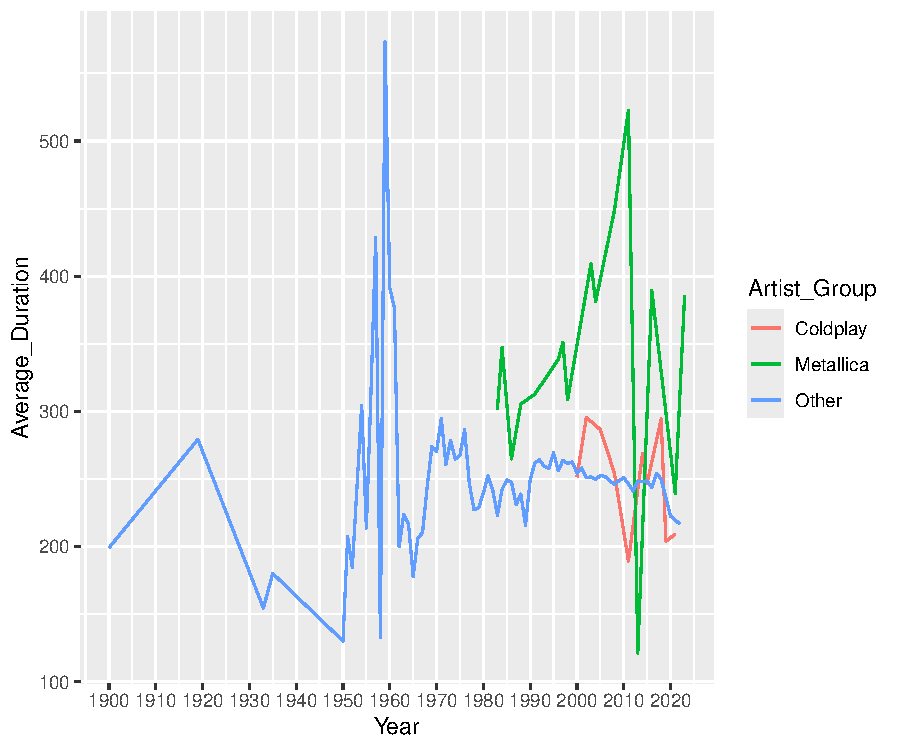
\includegraphics{Task_2_files/figure-latex/unnamed-chunk-4-1.pdf}

\subsection{Top 10 Most Popular Albums (Metallica
vs.~Coldplay)}\label{top-10-most-popular-albums-metallica-vs.-coldplay}

Moreover, the top 10 most popular albums of Metallica and Coldplay are
being visualized.

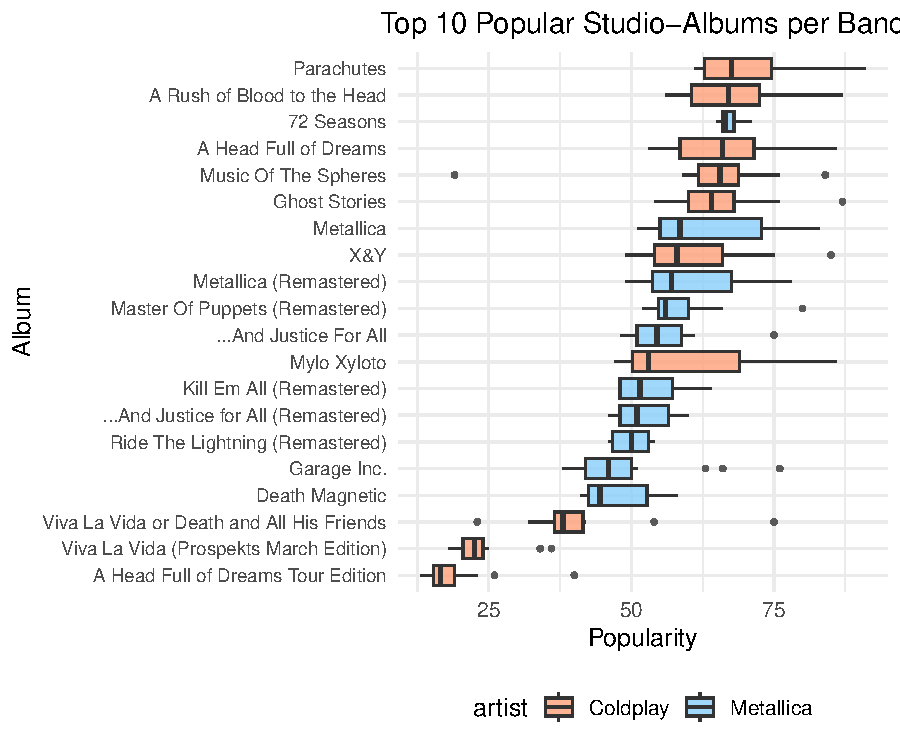
\includegraphics{Task_2_files/figure-latex/unnamed-chunk-5-1.pdf}

\subsection{Average Audio Features (Metallica
vs.~Coldplay)}\label{average-audio-features-metallica-vs.-coldplay}

Furthermore, average audio features of Metallica and Coldplay songs are
analysed and presented in a table.

\begin{longtable}[t]{clr}
\caption{\label{tab:unnamed-chunk-6}Comparison of Average Audio Features: Coldplay vs. Metallica}\\
\toprule
Feature & Coldplay & Metallica\\
\midrule
danceability & 0.427 & 0.414\\
energy & 0.562 & 0.798\\
loudness & -9.411 & -8.361\\
speechiness & 0.041 & 0.072\\
acousticness & 0.300 & 0.078\\
\addlinespace
instrumentalness & 0.254 & 0.374\\
liveness & 0.200 & 0.185\\
valence & 0.245 & 0.455\\
tempo & 126.610 & 122.162\\
duration & 243.591 & 304.211\\
\bottomrule
\end{longtable}

\subsection{Average Song Popularity (Metallica
vs.~Coldplay)}\label{average-song-popularity-metallica-vs.-coldplay}

In the next step, the average popularity of songs of Metallica and
Coldplay is being compared to get an understanding which of the bands is
more popular. The results suggest that Coldplay songs are on average
more popular, even though the band Metallica is longer standing and
hence more established on the music market than Coldplay.

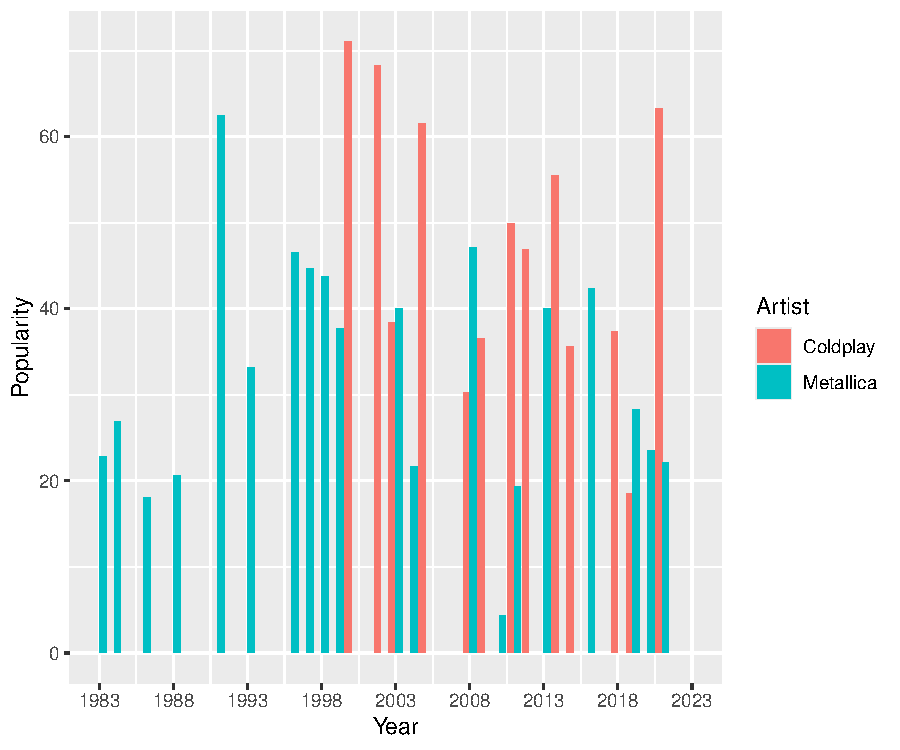
\includegraphics{Task_2_files/figure-latex/unnamed-chunk-7-1.pdf}

\subsection{Overview of Audio Features Over Time (Metallica vs.~Coldplay
vs.~Others)}\label{overview-of-audio-features-over-time-metallica-vs.-coldplay-vs.-others}

Lastly, average audio features of Metallica and Coldplay songs are
compared to average other songs over time. This allows to trace music
trends and evaluate whether the two bands are in line with overall
trends, as well as identify unique selling points of the bands. It
becomes apparent that Metallica is lowder and more energetic and live
than Coldplay and other artists. Coldplay is speechier and more
danceable and instrumental on average.

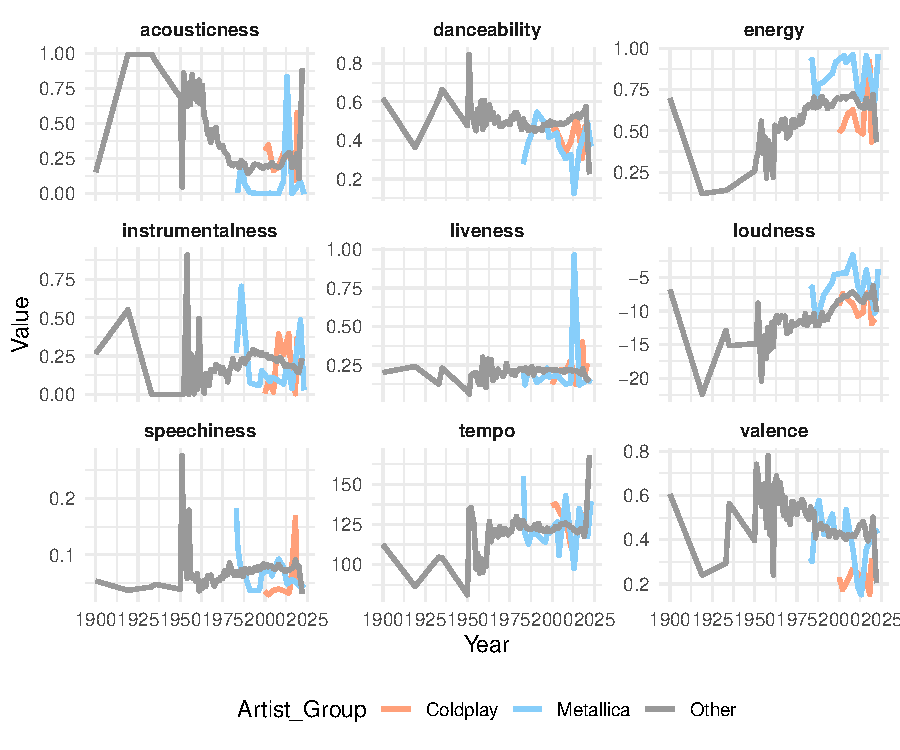
\includegraphics{Task_2_files/figure-latex/unnamed-chunk-8-1.pdf}

\section{Conclusion}\label{conclusion}

The analysis has shown that Coldplay songs are on average more popular
than Metallica ones. Furthermore, their music differs in the categories
under analysis (e.g.~energy, valence). Metallica songs tend to be longer
than Coldplay song and the average of other interprets songs. The
detailed audio feature analysis has shown that both bands have unique
selling points, differentiating their music from overall music trends
and average other bands.

\newpage

\bibliography{Tex/ref}





\end{document}
